%%%%%%%%%%%%%%%%%%%%%%%%%%%%%%%%%%%%%%%%%%%%%%%%%%%%%%%%%%          METAPODATKI

\begin{filecontents*}{\jobname.xmpdata}
\Title{Naslov magistrskega dela}
\Author{Ime in priimek}
\Keywords{magisterij\sep navodila\sep ključne besede}
\Publisher{Univerza v Ljubljani, Fakulteta za matematiko in fiziko}
\end{filecontents*}

%%%%%%%%%%%%%%%%%%%%%%%%%%%%%%%%%%%%%%%%%%%%%%%%%%%%%%%%%%

\documentclass[longbibliography,slovene,a4paper,12pt]{book}
%\usepackage[english]{babel}    % angleski delilni vzorci
\usepackage[slovene]{babel}    % slovenski delilni vzorci
\usepackage[utf8]{inputenc}
\usepackage{amsfonts}
\usepackage[T1]{fontenc}
\usepackage[pdftex]{graphicx}
\usepackage{fancyhdr}
\usepackage[sort, numbers]{natbib}

%%%%%%%%%%%%%%%%%%%%%%%%%%%%%%%%%%%%%%%%%%%%%%%%%%%%%%%%%%       PDF/A

\usepackage{xmpincl}
\usepackage[a-1b]{pdfx}       

%%%%%%%%%%%%%%%%%%%%%%%%%%%%%%%%%%%%%%%%%%%%%%%%%%%%%%%%%%

\usepackage{hyperref}
\usepackage[a4paper,inner=3.5cm,outer=2.5cm,top=2.5cm,bottom=2.5cm,pdftex]{geometry}
\usepackage[titletoc,title]{appendix}
\usepackage{epstopdf}
\usepackage{url}
\usepackage{makeidx}
\pagestyle{headings}
\makeindex

%%
%% Za pisanje sumnikov imamo tri moznosti:
%%   --- vnasamo jih neposredno v kodnem sistemu UTF-8 
%%   --- pisemo jih z latexovim ukazom, ki je namenjen natanko temu,
%%       in sicer kot \v{c}, \v{s}, \v{z}, \v{C}, \v{S}, v{\Z} ali
%%       malo manj pregledno kot \v c, \v s, \v z, \v C, \v S, \v Z,
%%   --- pisemo jih kot "c, "s, "z, "C, "S, "Z), vendar tedaj potrebujemo
%%       spodaj zapisani macro, ki znaku " pripise vlogo `izdelave' sumnika:
\catcode`\"=\active\def"#1{\v{#1}}
%%       torej \v{S}krjan\v{c}ek == \v Skrjan\v cek == "Skrjan"cek
%% Pozor: narekovaj potem ne smemo vec pisati kot " ampak kot `` in '',
%%       torej: "Skrjan"cek je "civkal ``"ci-"ci-"ci''.

%%
%% Mozni nacini stevilcenja strani:
%%  --- arabske stevilke v celotnem dokumentu, kot je uporabljeno v tej predlogi
%%  --- del strani je lahko stevilcen z rimskimi stevilkami, razen uvoda, osrednjega dela, zakljucka in seznama literature.
%% V vsakem primeru se stevilke na straneh izpisejo sele od kazala naprej.

\def\epsfg#1#2{\epsfig{file=#1.eps,width=#2}}
\def\legendamp#1#2{\vbox{\hsize=#1\caption{\small #2}}}

\setcounter{topnumber}{4}
\setcounter{bottomnumber}{4}
\setcounter{totalnumber}{5}
\renewcommand{\topfraction}{0.99}
\renewcommand{\bottomfraction}{0.99}
\renewcommand{\textfraction}{0.0}
\setlength{\tabcolsep}{10pt}
\renewcommand{\arraystretch}{1.5}

\def\bi#1{\hbox{\boldmath{$#1$}}}
\let\oldvec\vec
\def\vec#1{\mbox{\boldmath$#1$}}
\def\pol{{\textstyle{1\over2}}}
\def\svec#1{\mbox{{\scriptsize \boldmath$#1$}}}

\begin{document}

%%% NASLOVNA STRAN

\pagestyle{empty}
\begin{center}

{\large UNIVERZA V LJUBLJANI\\
FAKULTETA ZA MATEMATIKO IN FIZIKO\\
ODDELEK ZA FIZIKO\\
PROGRAM in SMER "STUDIJA\\}


\vspace{4cm}


{\Large Ime in priimek\\}

\vspace{10mm}

{\bf \Large NASLOV MAGISTRSKEGA DELA}\\
\vspace{5mm}
{\large Magistrsko delo}\\




\vfill



{\large MENTOR$\backslash$-ICA: naziv, Ime in priimek\\
SOMENTOR$\backslash$-ICA: naziv, Ime in priimek\\


\vspace{2cm}
Ljubljana, leto}

\end{center}

%%% ZAHVALA (NEOBVEZNO)

\cleardoublepage
\mbox{}
\vfill
{\Large \bf Zahvala}
\vspace{1cm}\\
Na tem mestu zapi"site, komu se zahvaljujete za pomo"c pri nastanku magistrskega dela.

%%% IZVLECEK

\cleardoublepage
{\Large \bf Izvle"cek}
\vspace{1cm}\\
Kratek izvle"cek v slovenskem jeziku.\\
\vspace{1cm}\\
{\bf Klju"cne besede:}\\
{\bf PACS:}

%%% ABSTRACT

\cleardoublepage
{\Large \bf Abstract}
\vspace{1cm}\\
Kratek izvle"cek v angle"skem jeziku.
\vspace{1cm}\\
{\bf Keywords:}\\
{\bf PACS:}

%%% KAZALO

\tableofcontents

%%% SEZNAM SLIK (NEOBVEZNO)

\cleardoublepage\phantomsection
\renewcommand\listfigurename{Seznam slik}
\addcontentsline{toc}{chapter}{\listfigurename}
\listoffigures

%%% SEZNAM TABEL (NEOBVEZNO)

\cleardoublepage\phantomsection
\renewcommand\listtablename{Seznam tabel}
\addcontentsline{toc}{chapter}{\listtablename}
\listoftables

\cleardoublepage

%%% OSREDNJI DEL

\pagestyle{fancy}
\fancyhead[CE,RE]{}
\fancyhead[LO,CO]{}
\fancyhead[LE]{\textbf{\nouppercase{\leftmark}}}
\fancyhead[RO]{\textbf{\nouppercase{\rightmark}}}

%\include{Uvod}

\chapter{Uvod}
\label{ch1}
Vzorec zaklju"cnega dela vsebuje najosnovnej"se elemente, 
ki jih lahko vklju"cimo v \LaTeX{}ov dokument. 
Ve"c o uporabi programa si lahko preberete na primer v 
\cite{Go}, \cite{Ba} ali \cite{Ra}. Na spletu je dostopna 
tudi "stevilna literatura v angle"skem jeziku. 
Dve med njimi sta \cite{ams}  in \cite{Gr}.

V tem vzorcu je za navajanje literature uporabljen program BibTeX. 
Ta je uporaben pri dalj"sem seznamu literature ali "ce avtor "zeli 
posamezne enote literature navesti tudi v svojih drugih delih. 
Seznam je urejen po vrstnem redu, kot se navedbe pojavijo v delu.
Seznam literature se pripravi v lo"ceni datoteki in se ga zato 
lahko uporabi v ve"c dokumentih.

\index{BibTeX}

Navajanje literature pa je mo"zno tudi v okolju {\tt thebibliography},
kjer posamezne enote na"stejemo ro"cno in v poljubnem vrstnem redu.
Uporaba okolja {\tt thebibliography} je opisana v navodilih za zaklju"cna dela.

Poglavje~\ref{ch2} opisuje vstavljanje matemati"cnih izrazov 
in ena"cb ter sklicevanje na ena"cbe. Poglavje~\ref{ch3} vsebuje 
slike in tabele, podnaslavljanje ter sklicevanje na njih.
Med besedilom so vklju"cene tudi opombe in citiranje literature.

%\include{Matemati"cni izrazi}

\chapter{Matemati"cni izrazi}
\label{ch2}

Spodnje besedilo je izsek iz u"cbenika J.~Strnada \cite{St}, 
kjer na straneh 35 in 36 navaja Newtonove zakone gibanja:

\section{Osnovne ena"cbe gibanja}
\subsection{Newtonovi zakoni}

Pri poskusih ugotovimo, da se giblje telo, na katerega deluje 
konstantna sila, enakomerno pospe"seno. Enaka sila povzro"ci 
vedno enak pospe"sek danega telesa.  Ugotovitve pri poskusih 
in druge izku"snje izrazimo z Newtonovimi zakoni~\footnote{~Zakone 
je objavil Isaac Newton 1687 v knjigi {\it Principia mathematica 
philosophiae naturalis.}  Prvi zakon je poznal "ze Galileo Galilei, 
ki ga je objavil 1638.}:

\begin{enumerate}
\item{Telo miruje ali se giblje premo enakomerno, "ce ne deluje nanj 
nobena sila.}
\item{Pospe"sek je sorazmeren s silo in ima smer sile.}
\item{"Ce deluje prvo telo na drugo telo s silo, deluje drugo telo 
na prvo z nasprotno enako silo.}
\end{enumerate}

Tretji zakon je znan kot zakon o vzajemnem u"cinku (zakon o akciji 
in reakciji). Drugi zakon zapi"semo z ena"cbo

\begin{equation}
{\bi F} = m {\bi a} \> .
\label{1NZ}
\end{equation}

Sila ${\bi F}$ je vektor, saj ima poleg velikosti tudi smer. 
Vektor pospe"ska ${\bi a}$ je vzporeden z vektorjem sile. 
Sorazmernostni koeficient  $m$ je masa.  To je koli"cina, 
ki meri vztrajnost telesa pri pospe"sevanju. Masa je v zvezi 
z mno"zino snovi.  Opazovanja in poskusi ka"zejo, da je masa aditivna: 
masa $m$ telesa, ki ga sestavimo iz telesa z maso $m_1$ in telesa 
z maso $m_2$, je enaka vsoti obeh mas:
$$
m = m_1 + m_2 \>.
$$
V Newtonovem zakonu (\ref{1NZ}) ne smemo videti definicije 
za silo ali definicije za maso. To je zakon narave, ki ga 
izlu"s"cimo iz opazovanj in poskusov.

%\include{Slike in tabele}

\chapter{Slike in tabele}
\label{ch3}

Slike in dalj"se tabele praviloma vklju"cujemo v dokument kot 
plavajo"ce objekte ali plovke (angle"sko floats).
Polo"zaj plovke v kon"cnem izdelku je odvisen od poteka besedila.
"Ce "zelimo dolo"citi to"cno mesto plovke, ukazu \verb|\begin{figure}|
ali \verb|\begin{table}| dodamo [dolo"cilo]:

\begin{itemize}
\item[---]{{\tt h} \hspace{1 cm} tukaj}
\item[---]{{\tt t} \hspace{1 cm} na vrhu strani}
\item[---]{{\tt b} \hspace{1 cm} na dnu strani}
\item[---]{{\tt p} \hspace{1 cm} na posebni strani}
\end{itemize}

\noindent
Slike in tabele potrebujejo podnapise s pojasnili. Vkolikor je slika povzeta iz drugega vira, mora biti tudi ta naveden:

\begin{figure}[h]
\begin{center}
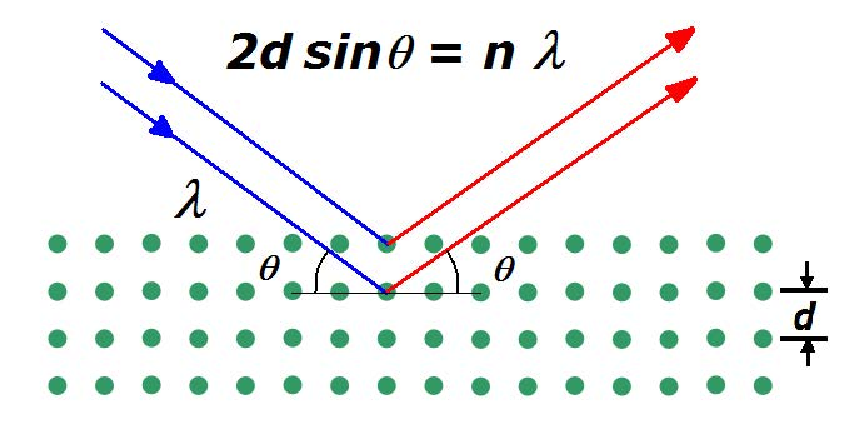
\includegraphics[width=10cm]{Bragglaw}
\end{center}
\caption[Braggov uklon.]{Braggov uklon je uklon oziroma sipanje 
rentgenskih "zarkov na kristalni mre"zi. Pri tem pride v dolo"cenih 
smereh zaradi interference do mo"cnih oja"canj. 
Slika je povzeta iz \cite{Bragg}.}
\label{pic1}
\end{figure}

\index{plovke}


Zaklju"cno delo lahko vsebuje kazalo slik in kazalo tabel. 
"Ce je podnapis predolg, da bi ga vklju"cili v kazalo, lahko 
namesto njega z ukazom \verb|\caption[...]{...}| med oglatima
oklepajema navedemo [skraj"sani podnapis], s katerim se bo slika 
ali tabela pojavila v kazalu.

\newpage
\section{Formati slik}

V \LaTeX{}ov dokument lahko vklju"cimo slike razli"cnih formatov. 
Vedeti pa moramo, da program {\tt pdflatex} podpira ve"c formatov 
kot {\tt latex}. Pri uporabi programa {\tt latex} lahko vstavljamo 
slike edino v formatu PostScript (.ps ali .eps --- kon"cnica ni
va"zna, le slika mora imeti definiran okvir, ki je zapisan
v njeni datoteki, obi"cajno v formatu \%\%{\tt BoundingBox x1 y1 x2 y2}). 
"Ce uporabljamo {\tt pdflatex}, so primerni formati na primer 
.png, .pdf in .jpg.  Tudi slike v formatu .eps je mo"zno vstaviti,
"ce tako kot v tem vzorcu uporabimo paket {\tt epstopdf}, ki vsako
.eps sliko samodejno pretvori v obliko .pdf.  (Lahko pa seveda
vsako .ps in .eps sliko "ze prej sami pretvorimo v sliko formata .pdf
z istim programom in uporabljamo le .pdf slike.  To je morda
celo najbolj priporo"cljiva pot.)  Strnjeno v Tabeli~\ref{tbl1}.

\begin{table}[h]
\caption[Dovoljeni formati slik]{Mimogrede: napisi k slikam so {\sl pod\/} slikami, 
napisi k tabelam so {\sl nad\/} tableami.  Ta tabela prikazuje
dovoljene formate slik.}
\label{tbl1}
\begin{center}
\begin{tabular}{l|ccc}
format & {\tt latex}  & {\tt pdflatex} \\ \hline
.pdf & ne  & da  \\
.png & ne  & da  \\
.jpg & ne & da  \\
.eps & da & da, pretvorjen z {\tt epstopdf} \\
.ps & da & da, pretvorjen z {\tt epstopdf}  \\
.bmp & ne & ne \\
.gif & ne & ne 
\end{tabular}
\end{center}
\end{table}

\index{pdflatex}

\chapter{Zaklju"cek}

Pisanje zaklju"cnega dela od vas zahteva veliko truda. 
Lotite se ga z veseljem, ob morebitnih vpra"sanjih 
ali te"zavah pa smo vam na voljo zaposleni na Oddelku za fiziko.

%%% LITERATURA

\cleardoublepage\phantomsection
\addcontentsline{toc}{chapter}{Literatura}
\bibliographystyle{myapsrevSLO}
\bibliography{Bibliografija}

%%% DODATKI

\cleardoublepage
\renewcommand\appendixname{Dodatek}
\begin{appendices}

\chapter{Naslov prvega dodatka}
    
Dodatek je samostojna vsebina, ki ne sodi v osrednji del besedila. 
Ima svoj naslov in pravilno je, da se nanj v besedilu vsaj enkrat sklicujemo.
V dodatek spadajo na primer zahtevnej"se izpeljave, dalj"se tabele 
ali seznami ter vsebine, ki niso neposredno povezane z osrednjim besedilom. 
"Ce je dodatkov ve"c, jih ozna"cimo s "crkami: Dodatek A, Dodatek B itd.

\chapter{Naslov drugega dodatka}
    
V pomo"c pri pisanju znanstvenega besedila vam je lahko na primer knjiga \cite{All}.

\end{appendices}

%%% KAZALO (NEOBVEZNO)

\cleardoublepage
\printindex

\end{document}